\documentclass{article}[a4paper]
\usepackage[a4paper, total={6.5in, 9in}]{geometry}
\usepackage{float}
\usepackage{amsmath}
\usepackage{amssymb}
\usepackage{enumitem}
\usepackage{tabularray}
\usepackage{charter}
\usepackage{xcolor}
\usepackage{graphicx}
\usepackage{listings}
\usepackage{tikz}
\usepackage{parskip}
\usepackage{tcolorbox}
\usepackage[hidelinks]{hyperref}
\tcbuselibrary{breakable}

\allowdisplaybreaks

\newcommand{\extlink}{
	
\begin{tikzpicture}[scale=0.1]
		\draw[rounded corners=0.5mm, line width=0.9pt] (-1, -1) rectangle (1, 1);
		\fill[white] (0, 0) rectangle (1.3, 1.3);
		\draw[line width=0.9pt, line cap=round] (0.15, 0.15) -- (1.3, 1.3);
		\draw[line width=0.9pt, line cap=round] (0.5, 1.3) -- (1.3, 1.3) -- (1.3, 0.5);
	\end{tikzpicture}
}

\lstset{
	language=Matlab,
	basicstyle=\ttfamily,
	keywordstyle=\color{blue},
	commentstyle=\color{gray},
	stringstyle=\color{red},
	showstringspaces=false,
	columns=fullflexible,
	breaklines=true,
	captionpos=b,
	backgroundcolor=\color[rgb]{0.96,0.96,0.96},
	xleftmargin=6pt,
	frame=tlbr,
	framesep=6pt,
	framerule=0pt,
}

\tcbset{width=\linewidth, boxrule=0pt, colframe=white, colback=white, breakable, boxsep=0pt, left=0pt, right=0pt}

\setlist[itemize]{itemsep=2pt, parsep=3pt}

\title{
	\huge{\textbf{
		Assignment 02
	}}\\
	\large{\phantom{}}\\
	\large{
		submitted for
	}\\
	\Large{
		\textbf{EN3551 - Digital Signal Processing}
	}\\
	\large{
		Department of Electronic and Telecommunication Engineering
	}
	\\
	\large{University of Moratuwa}
}

\author{
	\textbf{Udugamasooriya P. H. J.}\\
	220658U\\
	\small{Progress on \href{https://github.com/pulasthi-u/en3551-assignment02}{GitHub \extlink}}
}

\date{26 October 2025}

\begin{document}
	\maketitle

	\textbf{Question 03} The relevant images and quality levels are \texttt{cameraman.mat}, \texttt{Monarch.mat}, \texttt{Parrot.mat}, and 80\%, 30\% and 15\%. We compress and decompress each image and compare with the original image at each of the quality levels given.
	
	Note that we skip the process of coding and decoding, as we are only interested in the effects of compression on the visual quality of the image.
	
	Results obtained for each image are as follows:
	
	\begin{enumerate}
		\item \texttt{cameraman.mat}
		
		\begin{tcolorbox}
			\begin{figure}[H]
				\centering
				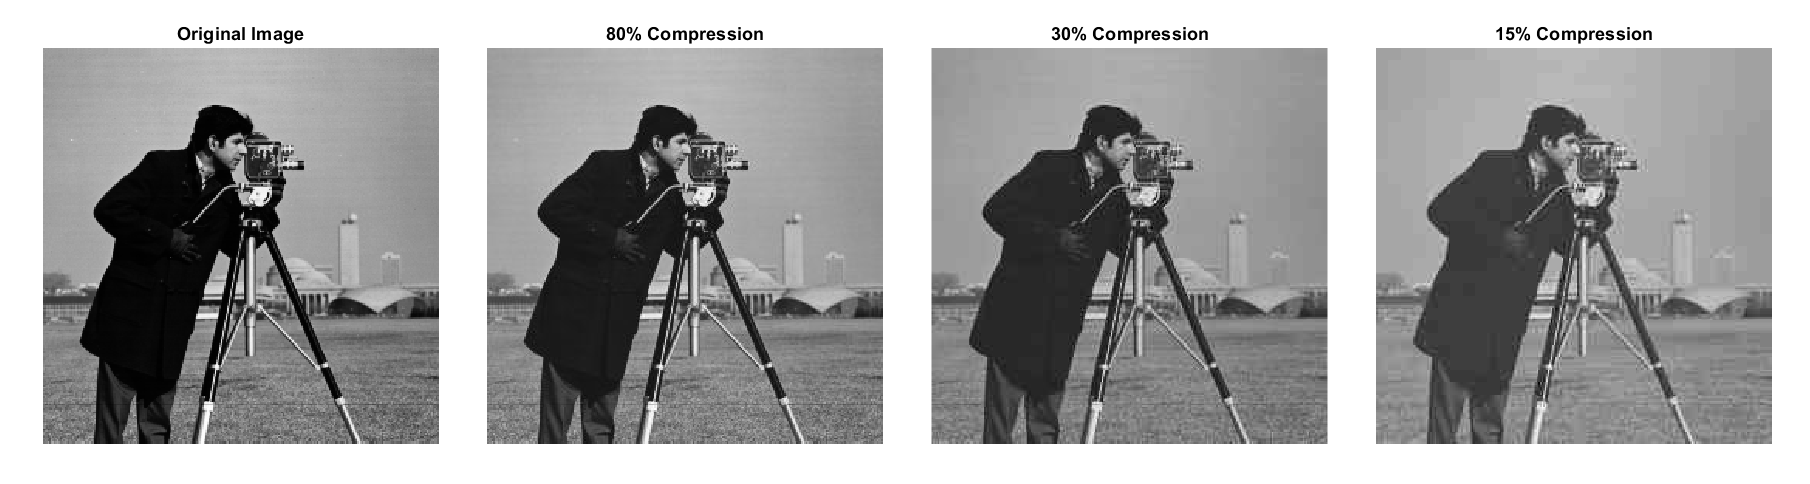
\includegraphics[width=\linewidth]{images/cameraman.png}
				\caption{\texttt{cameraman.mat} at various compression levels}
				\label{cameraman}
			\end{figure}
		\end{tcolorbox}
		
		\begin{tcolorbox}
			\begin{table}[H]
				\begin{tblr}{
						colspec={XXXX},
						vlines, hlines
					}
					Quality Level		& 80\% & 30\% & 15\% \\
					Percentage of Zeros	& 74.9786\% & 89.386\% & 93.3502\% \\
					PSNR (dB)			& 35.7235 & 29.6951 & 27.4598 \\
				\end{tblr}
			\end{table}
			
			Comments on visual quality:
			\begin{itemize}
				\item 80\% compression
				\begin{itemize}
					\item virtually indistinguishable from the original
					\item slight reduction in contrast levels, e.g., the coat is grayer than in the original
				\end{itemize}
				\item 30\% compression
				\begin{itemize}
					\item slight blockiness is visible, especially towards the upper right
					\item some ringing is visible at the edges; there is a slight halo around the cameraman and camera
					\item the grass on the ground appears blurry
				\end{itemize}
				\item 15\% compression
				\begin{itemize}
					\item significant blockiness is visible
					\item ringing effects are visible---there is a blurry halo around the cameraman and camera
					\item the grass on the ground is significantly more blurry
					\item there is a clear reduction in contrast levels
				\end{itemize}
			\end{itemize}
		\end{tcolorbox}
		
%		\begin{minipage}{\linewidth}
%			
%		\end{minipage}
		\vspace{0.5 em}
		
		\item \texttt{Monarch.mat}
		
		\begin{tcolorbox}
			\begin{figure}[H]
				\centering
				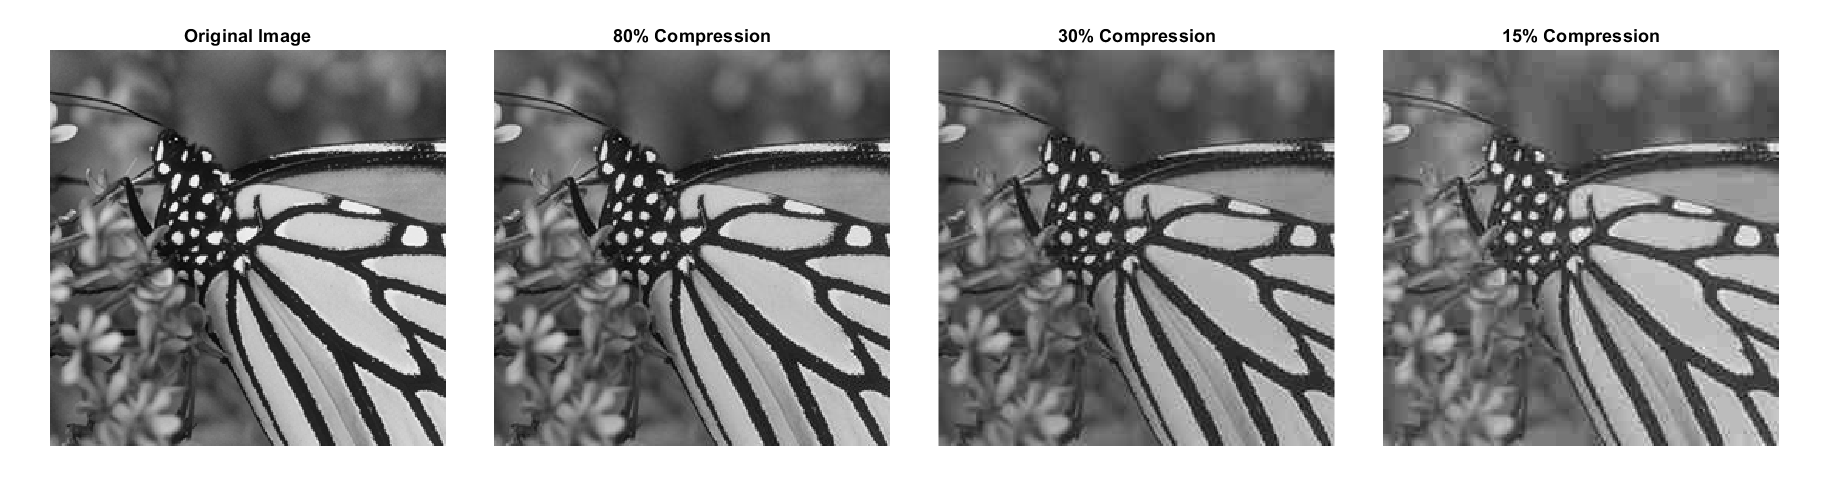
\includegraphics[width=\linewidth]{images/monarch.png}
				\caption{\texttt{Monarch.mat} at various compression levels}
				\label{monarch}
			\end{figure}
		\end{tcolorbox}
		
		\begin{tcolorbox}
			\begin{table}[H]
				\begin{tblr}{
						colspec={XXXX},
						vlines, hlines
					}
					Quality Level		& 80\% & 30\% & 15\% \\
					Percentage of Zeros	& 71.8948\% & 85.7666\% & 90.2161\% \\
					PSNR (dB)			& 35.7556 & 30.0778 & 27.725 \\
				\end{tblr}
			\end{table}
			
			Comments on visual quality:
			\begin{itemize}
				\item 80\% compression
				\begin{itemize}
					\item virtually indistinguishable from the original
					\item slight reduction in contrast levels, e.g., the black lines in the wings seem a lighter shade of gray and the brighter, white regions seem more dull
				\end{itemize}
				\item 30\% compression
				\begin{itemize}
					\item blockiness is visible
					\item further reduction in contrast levels
				\end{itemize}
				\item 15\% compression
				\begin{itemize}
					\item significant blockiness is visible
					\item the outlines around the white regions on the wings are no longer sharp and have blurred out
				\end{itemize}
			\end{itemize}
		\end{tcolorbox}
		\vspace{0.5 em}
		
		\item \texttt{Parrot.mat}
		
		\begin{tcolorbox}
			\begin{figure}[H]
				\centering
				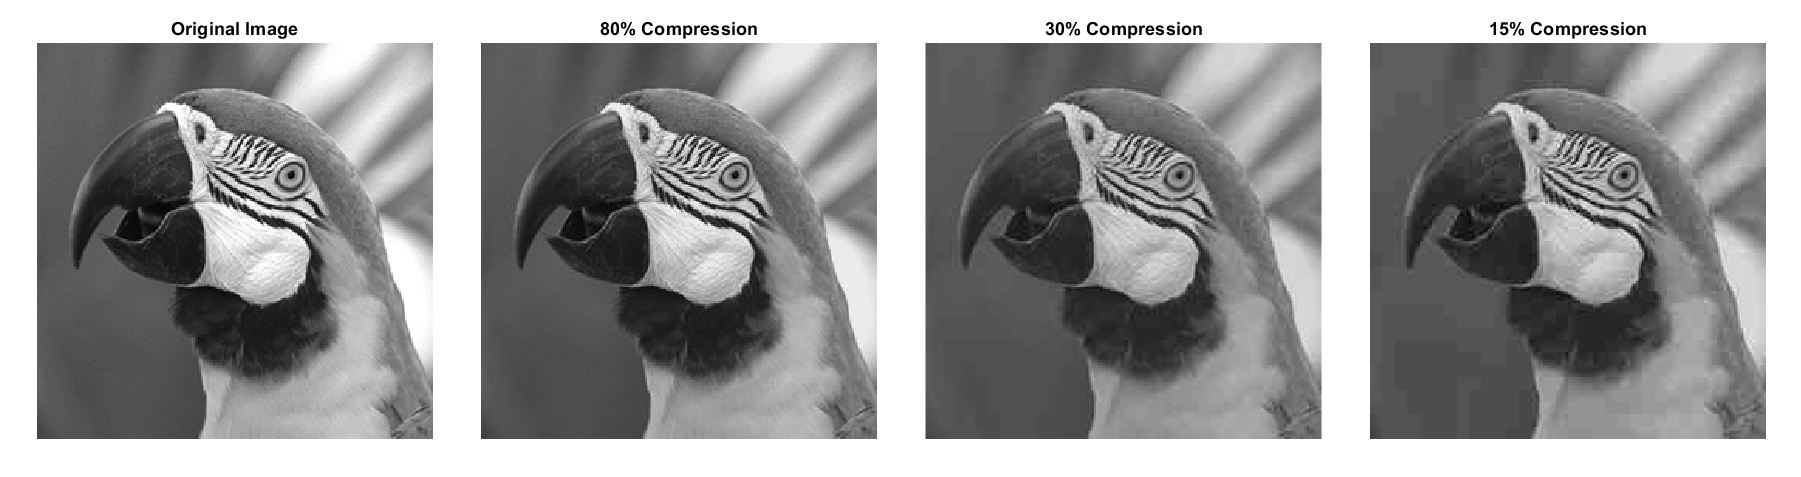
\includegraphics[width=\linewidth]{images/parrot.png}
				\caption{\texttt{Parrot.mat} at various compression levels}
				\label{parrot}
			\end{figure}
		\end{tcolorbox}
		
		\begin{tcolorbox}
			\begin{table}[H]
				\begin{tblr}{
						colspec={XXXX},
						vlines, hlines
					}
					Quality Level		& 80\% & 30\% & 15\% \\
					Percentage of Zeros	& 80.5573\% & 91.2155\% & 94.1544\% \\
					PSNR (dB)			& 38.2348 & 32.9118 & 30.4194 \\
				\end{tblr}
			\end{table}
			
			Comments on visual quality:
			\begin{itemize}
				\item 80\% compression
				\begin{itemize}
					\item very similar to the original
					\item fine details of the feathers have diminished
				\end{itemize}
				\item 30\% compression
				\begin{itemize}
					\item further blurring of the details of feathers
					\item some blockiness visible
				\end{itemize}
				\item 15\% compression
				\begin{itemize}
					\item significant blockiness is visible
					\item significant loss of detail of the feathers; the body seems made up of plain colors
					\item slight halo visible near the back of the neck
				\end{itemize}
			\end{itemize}
		\end{tcolorbox}
		\vspace{0.5 em}
		
		\newpage
		
		\item Image of Choice - \texttt{pisa.jpg}
		
		\begin{tcolorbox}
			\begin{figure}[H]
				\centering
				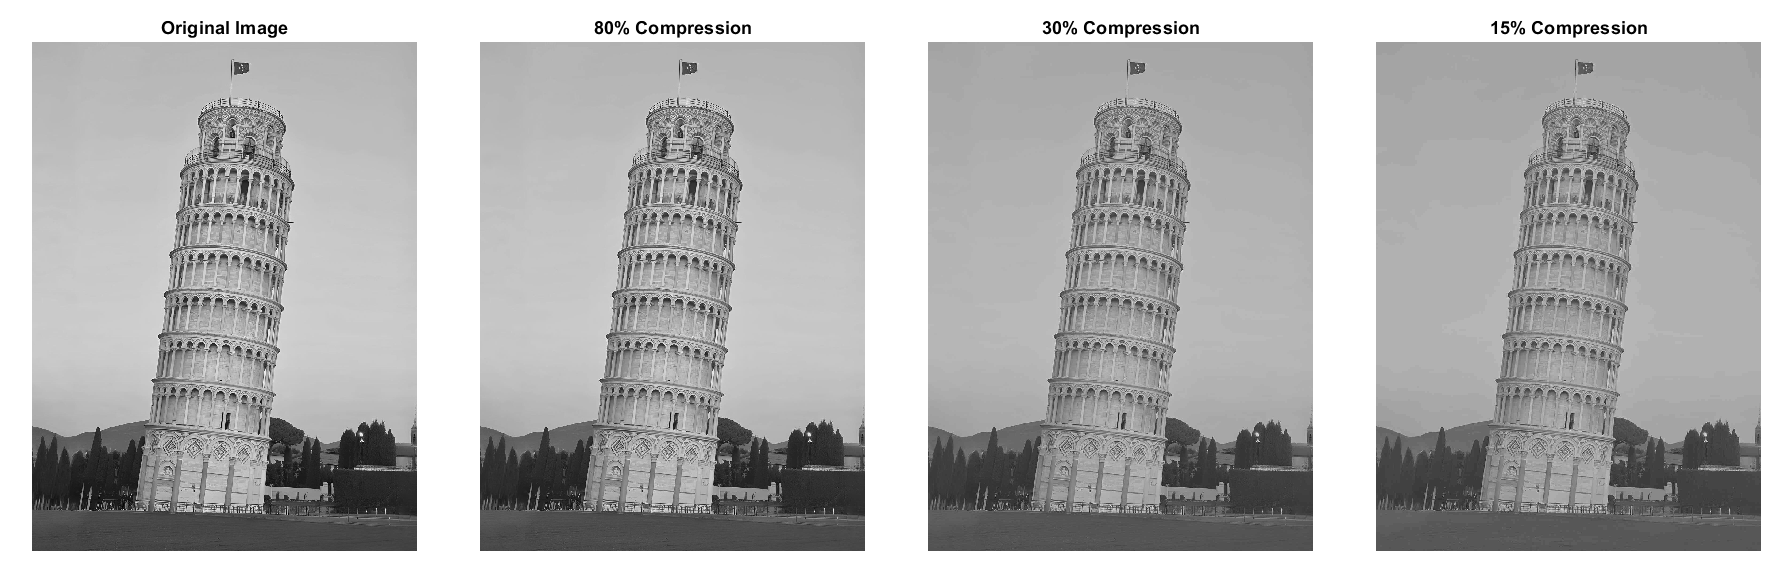
\includegraphics[width=\linewidth]{images/pisa.png}
				\caption{\texttt{pisa.jpg} at various compression levels}
				\label{pisa}
			\end{figure}
		\end{tcolorbox}
		
		\begin{tcolorbox}
			\begin{table}[H]
				\begin{tblr}{
						colspec={XXXX},
						vlines, hlines
					}
					Quality Level		& 80\% & 30\% & 15\% \\
					Percentage of Zeros	& 87.8315\% & 93.783\% & 95.6683\% \\
					PSNR (dB)			& 42.1905 & 34.3926 & 31.6468 \\
				\end{tblr}
			\end{table}
			
			Comments on visual quality:
			\begin{itemize}
				\item 80\% compression
				\begin{itemize}
					\item virtually indistinguishable from the original
				\end{itemize}
				\item 30\% compression
				\begin{itemize}
					\item walls seem smoothed out
					\item fine details of carvings and engravings are not visible and are blurry
				\end{itemize}
				\item 15\% compression
				\begin{itemize}
					\item further loss of fine details due to blurring out
					\item bands visible in the sky instead of a smooth transition between colors
					\item some blockiness visible in the grass
				\end{itemize}
			\end{itemize}
		\end{tcolorbox}
	\end{enumerate}
	
	We wish to also make the following general comments:
	\begin{itemize}
		\item The quantity $\sigma_e$ is a measure of the average variability/error between the original image and reconstructed image.
		
		The PSNR measures how $\sigma_e$ compares with the maximum intensity level $\psi_\text{max}$ in the image.
		
		If $\dfrac{\psi_\text{max}}{\sigma_e}$ is high, then we expect the intensity levels in the reconstructed image to remain very close to those of the original image, but to deviate more significantly otherwise.
		
		In each of the images, the PSNR can be seen to decrease with decreasing quality level, as expected.
		
		\item In each of the cases, even with a quality level as high as 80\%, we see that the algorithm has managed to reduce more than 70\% of the entries in the matrix to zeros, giving a very significant compression at negligible loss of visual quality.
	\end{itemize}
	
	\newpage
	
	\textbf{Question 04} We will compare the compressed images over the quality level 15\%.
	
	Across the three given images, it seems that \texttt{Monarch.mat} shows the most degradation, followed by \sloppy\texttt{cameraman.mat}, and \texttt{Parrot.mat} shows the least degradation.
	
	Further, it seems that the image of personal choice, \texttt{pisa.jpg}, shows even less degradation than \texttt{Parrot.mat}.
	
	Among the first three images, \texttt{Monarch.mat} has the most activity, i.e., high frequency content, compared to the other two. Further, \texttt{cameraman.mat} has some sharp edges whereas \texttt{Parrot.mat} mostly has smoother edges.
	
	This explains the disparity among their compressed versions. The effect of the DCT is to suppress high frequency content from an image, so images with a lot of such detail will undergo heavier degradation for the same quality level.
	
	As sharp edges also contribute high frequency content to an image, images with such edges will also tend to degrade more than images with softer edges. We expect to see some ringing around such edges in the reconstruction due to the suppressed high frequencies.
	
	We note that even though an image might contain quickly changing features/textures, if they are concentrated to small regions of the image, or if the features are small compared to the main subject of the image, the loss in such detail appears unnoticeable.
	
	For example, the detail of the parrot's feathers, while constituted of high frequencies, remains mostly unnoticeable even in the original image, unless one inspects very closely. However, high frequency content is spread all throughout the image of the butterfly, due to the rapidly varying patterns on its wings.
	
	Hence, the loss of detail in the butterfly's wings is more apparent in the compressed image than the loss of detail in the parrot's feathers.
	
	Another observation made is the appearance of bands in the compressed image when the original contains smooth gradients. This is a consequence of the choice of independently quantizing 8$\times$8 blocks of the image.
	
	The 8$\times$8 blocks restrict the frequencies that can be used to represent the variation within a block to those of cosines taking the form \[\cos\left(\dfrac{(2n+1)k\pi}{16}\right).\] However, when the image size is much larger than $8\times8$, it could contain gradients with far lower frequencies than could be represented by such cosines.
	
	As a result, it is possible that such blocks be approximated solely by the average pixel value within them. This could lead to the formation of bands.
	
	These effects are visible in the background of \texttt{cameraman.mat} and \texttt{pisa.jpg}, and more significantly so in \texttt{pisa.jpg} due to its greater height.
	
	\appendix
	\section{Code Snippets}
	\label{code}
	
	\begin{lstlisting}[caption={Main Code}, label=harmonic_main]
clear;
clc;
close all;

% 3.1.1 - Load the relevant signal
load('signal658.mat');

% Define useful constants
fs = 128; % Sampling frequency (given)
Ns = [128 256 512 1024 1792]; % Sizes of subsets to be formed (given)

% For plotting
figure(1);
tiledlayout(3, 2, "TileSpacing", "compact", "Padding", "compact");

% Try to detect harmonics from the DFTs of increasingly bigger subsets of
% the signal

for i = 1:5
	N_i = Ns(i); % Number of samples in the ith subset
	f_i = [0:(N_i-1)] * fs / N_i; % Frequency axis corresponding to the ith subset
	
	% 3.1.2 - Form the ith subset s_i
	s_i = xn_test(1:N_i);
	
	% 3.1.3 - Obtain the DFT S_i of the ith subset, and then its magnitude
	S_i = fft(s_i);
	S_i_mag = abs(S_i);
	
	% We will plot the first four figures in a 2x2 configuration, with the
	% last one in a row of its own
	if i <= 4
	nexttile(i);
	else
	nexttile(i, [1, 2]);
	end
	
	% 3.1.3 - Plot the magnitudes of the DFT of the ith signal
	stem(f_i, S_i_mag, "Marker", "o", "MarkerSize", 3, "MarkerFaceColor", "auto");
	
	title("DFT-Magnitude of $S_" + i + "$", "Interpreter", "latex");
	xlabel("Frequency (Hz)", "Interpreter", "latex");
	xlim([0 f_i(N_i)]);
	grid on;
	grid minor;
end

% Try to detect harmonics by averaging

L = 14; % Number of subsets
K = 128; % Number of samples in a subset

% 3.1.4 - Find the average DFT from L = 14 consecutive subsets of K = 128
% samples each, and then obtain its magnitude
X_avg = dft_average(xn_test, L, K);
X_avg_mag = abs(X_avg);

f = [0:(K-1)] * fs / K; % Define the frequency axis

% Plot the magnitude of the average DFT
figure(2);

stem(f, X_avg_mag, "Marker", "o", "MarkerSize", 3, "MarkerFaceColor", "auto");

title("Magnitude of Averaged DFTs", "Interpreter", "latex");
xlabel("Frequency (Hz)", "Interpreter", "latex");
xlim([0 f(K)]);
grid on;
grid minor;

% 3.1.5 - What is the smallest value of L such that the peaks remain
% visible?

figure(3);
tiledlayout(3, 2);

% We will try smaller values L_s for L, starting from 1 less than the last
% used value
for L_s = [13 10 8 7 6 5]
	% Obtain the average DFT for the chosen pair L_s, K
	X_avg_ = dft_average(xn_test, L_s, K);
	X_avg_mag_ = abs(X_avg_);
	
	nexttile;
	
	% Plot
	stem(f, X_avg_mag_, "Marker", "o", "MarkerSize", 3, "MarkerFaceColor", "auto");
	
	title("Average DFT Magnitude, $L=" + L_s + "$, $K=" + K + "$", "Interpreter", "latex");
	xlabel("Frequency (Hz)", "Interpreter", "latex");
	xlim([0 f(K)]);
	grid on;
	grid minor;
end
	\end{lstlisting}
	
	\begin{lstlisting}[caption={DFT averaging}, label=dft_avg_code]
function [result] = dft_average(x, L, K)
% DFT_AVERAGE Average DFT of L consecutive subsets of K samples each from x
%   x   =   time-domain signal
%   L   =   number of subsets
%   K   =   number of samples from each subset
%
% Computes the DFT of L consecutive K-point signal formed by partitioning
% x, and returns the average; i.e., sum of the DFTs divided by L

% We compute the DFTs of K-point signals; they will have K samples
% themselves; construct a dummy K-dimensional array to store the result
result = complex(zeros(1, K));

for j = 0:(L-1)
	x_j = x(j*K+1:(j+1)*K); % jth subset
	X_j = fft(x_j); % DFT of the jth subset
	
	% Keep accumulating the DFT over subsets
	result = result + X_j;
end

% Average the DFT
result = result / L;

end
	\end{lstlisting}
	
	\subsection{Interpolation}
	\begin{lstlisting}[caption={Main Code}, label=interpol_main]
clear;
clc;
close all;

% 3.2.1 - Load the signal
load handel;

% We will only be looking at the first 20,000 samples of the signal
N = 20000;
x_1 = y(1:N);

% Visualize the original signal
figure;

stem(x_1(1:50), "Marker", "o", "MarkerSize", 3, "MarkerFaceColor", "auto");

title("Original Signal", "Interpreter", "latex");
grid on;
grid minor;

% Empty array to store interpolations for later comparison
interpolations = {};

for i = 2:4
	% 3.2.2 - Form the signal x_i as described
	x_i = y(1:i:N);
	
	% 3.2.3 -
	% Obtain an interpolated version of x_i from the zero-padded DFT of x_i
	% with K = i - 1
	x_i_interpolated = interpolate(zero_padded_dft(x_i, i-1), i-1);
	
	% Compute the norm of the difference between the original signal and
	% the interpolated version
	disp("Norm of difference: " + difference_norm(x_i_interpolated, x_1));
	
	% Plot the signals for comparison
	plot_interpolation_v_actual(x_i_interpolated, x_1);
	
	% Save the current interpolated version for later comparison
	interpolations{end+1} = x_i_interpolated;
end

% Plot all interpolated signals together, and on top of each other with the
% original signal for comparison
figure;

% Plot the original signal
subplot(5, 1, 1);

stem(x_1(1:50), "Marker", "o", "MarkerSize", 3, "MarkerFaceColor", "auto");

title("Original Signal", "Interpreter", "latex");
grid on;
grid minor;

% Plot each interpolated signal in succession
for i = 1:3
	subplot(5, 1, i + 1);
	
	interpolation_i = interpolations{i};
	stem(interpolation_i(1:50), "Marker", "o", "MarkerSize", 3, "MarkerFaceColor", "auto");
	
	title("$x_" + (i+1) + "$ Interpolated", "Interpreter", "latex");
	grid on;
	grid minor;
end

% Plot all interpolations and the original signal on top of each other
subplot(5, 1, 5);

stem(x_1(1:50), "Marker", "o", "MarkerSize", 3, "MarkerFaceColor", "auto");
hold on;

for j = 1:3
	interpolation_j = interpolations{j};
	stem(interpolation_j(1:50), "Marker", "o", "MarkerSize", 2+j);
	hold on;
end

title("Comparison", "Interpreter", "latex");
legend("Original Signal", "$x_2$ Interpolated", "$x_3$ Interpolated", "$x_4$ Interpolated", "Interpreter", "latex");
grid on;
grid minor;

% Helper Functions

function [] = plot_interpolation_v_actual(interpolation, actual)
	figure;
	
	% Plot the interpolated signal
	subplot(2, 1, 1);
	
	stem(interpolation(1:50), "Marker", "o", "MarkerSize", 3, "MarkerFaceColor", "auto");
	
	title("Interpolated Signal", "Interpreter", "latex");
	grid on;
	grid minor;
	
	% Plot the interpolated signal on top of the actual signal for
	% comparison
	subplot(2, 1, 2);
	
	stem(interpolation(1:50), "Marker", "o", "MarkerSize", 3, "MarkerFaceColor", "auto");
	hold on;
	stem(actual(1:50), "Marker", "o", "MarkerSize", 5);
	
	title("Interpolated Signal vs. Actual Signal", "Interpreter", "latex");
	legend("Interpolated Signal", "Actual Signal");
	grid on;
	grid minor;
end

function [result] = difference_norm(x1, x2)
	% Find the length of the shorter signal
	N = min(length(x1), length(x2));
	
	% Truncate both signals to the same length
	x1_trunc = x1(1:N);
	x2_trunc = x2(1:N);
	
	% Compute the norm of the difference between the truncated signals
	result = norm(x1_trunc - x2_trunc);
end
	\end{lstlisting}
	
	\begin{lstlisting}[caption={Zero-padding DFT}, label=zero_pad_dft_cod]
function [result] = zero_padded_dft(x, K)
% ZERO_PADDED_DFT Obtain an (K+1)N-point DFT of x with zeros inserted in
% the middle
% 
%   x   =   time-domain signal, of length N
%   K   =   sets the length of the resulting DFT
%
% Compute the DFT of x, split it in the middle, insert zeros between the
% two halves, and return the result. Splitting and other manipulations are
% done depending on the parity of N.

% Start by obtaining the DFT of x
X = fft(x);
N = length(X);

if mod(N, 2) % If X has an odd number of samples
	n = (N+1)/2; % Index of the point to split from
	
	% Insert KN zeros as described
	result = [
		X(1:n);
		complex(zeros(K*N, 1));
		X((n+1):N)
	];
else % If X has an even number of samples
	n = N/2; % Index of the point to split from
	
	% Insert KN - 1 zeros as described
	result = [
		X(1:n);
		X(n+1)/2;
		complex(zeros((K*N)-1, 1));
		X(n+1)/2;
		X((n+2):N)
	];
end

end
	\end{lstlisting}
	
	\begin{lstlisting}[caption={Interpolation}, label=interp_code]
function [result] = interpolate(X, K)
%INTERPOLATE

N = length(X)/(K+1);

x = (K+1) * ifft(X);

result = x(1:((K+1)*(N-1)+1));

end
	\end{lstlisting}
\end{document}